\section{Proof Automation}\label{automated-sec}

In this project we used proof automation in two ways: automated theorem provers (ATPs) and Lean tactics.
ATPs are generally stand-alone tools that implement a (semi-) decision procedure for a given formal language or related set of languages.
For example, Vampire~\cite{DBLP:conf/cav/KovacsV13} is an ATP focused primarily on first-order logic using superposition, which we used extensively in this project.

ATPs are complex software that can contain bugs.
Instead of trusting ATP output, we used proof certificates, which many ATPs can produce, to reconstruct a proof in Lean.
This process depends on the proof certificate and the ATP, and we describe it for the main reconstruction we have done.

Tactics in Lean, on the other hand, are meta-programs~\cite{DBLP:journals/pacmpl/EbnerURAM17} that builds proofs.
In other words, tactics are programs that operate at the meta-level of Lean code: they essentially take in Lean code as input and produce Lean code as output.
In this manner, they look like another keyword in the language, and are tightly integrated by producing proofs directly.
Under the hood, they can implement essentially anything, from syntactic sugar to full decision procedures.
The \texttt{duper} tactic~\cite{DBLP:conf/itp/CluneQBA24}, for example, implements a superposition calculus, similar to Vampire's, but for dependent types --- Lean's underlying logical foundation.

In the rest of this section we describe the different proof automation techniques and ATPs/tactics we used.
We first discuss the different proof methods used: primarily superposition and equational reasoning, we then discuss the integration in Lean, and finally we report some basic empirical results from this project.

\subsection{Proof Techniques}

The main two families of ATPs and tactics we used here are superposition/saturation-based and equational reasoning ones.
In this context we also include SMT solvers, which combine specific decision procedures for theories, like congruence closure for equational reasoning, with satisfiability (SAT) solving \note{Give citation}.
Finally, we also used \texttt{aesop}~\cite{DBLP:conf/cpp/LimpergF23}, which implements a version of tableau search.
This was used mainly to help specific constructions in refutations, and is not specific to proving or disproving magma implications in this sense.
We will describe our use of \texttt{aesop} more in \Cref{sec:proof-reconstruction} below.

\paragraph{Saturation}
Most of the ATPs we used extensively in this project rely primarily on saturation procedures in the superposition calculus.
This is the case for Vampire~\cite{DBLP:conf/cav/KovacsV13}.
See also~\cite{DBLP:journals/cacm/BentkampBNTVW23} for a gentler exposition.
The core idea of these provers is that they take a set of assumptions with a conjecture, expressed in --- say --- first-order logic.
They take the conjecture and negate it, adding this negation to the set of assumptions, which are all put in some normal form.
The ATP then tries to refute the negation by applying rules of the underlying calculus, until they find a proof of false (a contradiction).
In this case, the conjecture was (classically) true, and the ATP has found a proof by contradiction, often called a ``refutation'' or ``saturation'' proof.

The underlying calculus varies from system to system, but they often have a variant of a resolution clause, a clause of a form:
\[\infer{C \lor D}{C \lor L \quad D \lor \neg L} \]
This can also be read as $C \lor L$ with $D \lor \neg L$ implies $C \lor D$, where $C, D, L$ are formulas in e.g. first-order logic.
Superposition calculi have a variant of this rule that deals with equality directly, and thus are more efficient at reasoning about equality.

In this project we used Vampire~\cite{DBLP:conf/cav/KovacsV13}, Duper~\cite{DBLP:conf/itp/CluneQBA24} and Prover9 and Mace4~\cite{prover9-mace4} which are all based on variants of saturation for proving.
TODO: here we could add a screenshot of using vampire or prover9.

\paragraph{Equational Reasoning}

Equational reasoning is a type of reasoning based on equational logic and rewriting with congruence~\cite{term-rewriting}, see Chapter ??? for a discussion of its foundations in universal algebra.
In general, it takes a series of equations and determines whether another equation can be deduced from it.
A core tool in equational reasoning are e-graphs, a data structure used to represent equivalence classes of terms.
The procedure of congruence closure that can be used to decide ground equational problems (i.e. problems without variables) and as a semi-decision procedure in general.

SMT solvers like Z3~\cite{DBLP:conf/tacas/MouraB08} use equational reasoning for deciding the theory of equality with uninterpreted functions~\cite{DBLP:series/txtcs/KroeningS16,DBLP:conf/cade/MouraB07}.
On the other hand, equality saturation~\cite{DBLP:journals/pacmpl/WillseyNWFTP21} uses e-graphs by extending congruence closure to a more controlled search, enabling optimization and conditional rewriting.
One of the main advantages of using equational reasoning to reason about implications of magma laws is that we get very explicit proofs: a proof that $l \vdash l'$ is given by a sequence of rewrites that starts at the left-hand side of $l'$ and arrives at the right-hand side through applications of $l$.

In this project we used Z3~\cite{DBLP:conf/tacas/MouraB08}, Prover9 and Mace4~\cite{prover9-mace4}, a custom ATP for magmas based on egg~\cite{DBLP:journals/pacmpl/WillseyNWFTP21}, and the Lean egg tactic~\cite{DBLP:journals/pacmpl/KoehlerGBGTS24,rossel2024bridging}, which all work with equational logic. We have also reasoned with manual (custom written) heuristics about simple rewrites.

\subsection{Proof Reconstruction and Integration}
\label{sec:proof-reconstruction}

While ATPs are very useful to solve questions for this project, they generally don't integrate well with Lean.
A bug in an ATP could lead to an unsound proof, or worse, an incorrect result.
To avoid having to trust ATP's large codebases, we take results found by the different provers and (re-)construct their proofs in Lean.

An exception for this are tactics like \texttt{duper}, \texttt{aesop} and \texttt{egg}. Figure~\ref{fig:screenshot-egg} shows an example of the \texttt{egg} tactic as used in this project. It integrates directly in Lean, generating a Lean proof directly. With the variant \texttt{egg?}, depicted in the screenshot, it uses an auxiliary tactic \texttt{calcify}\footnote{\url{https://github.com/nomeata/lean-calcify}} to generate a human-readable proof as a series of calculation steps, which can be incorporated into the file with a single click.

\begin{figure}
  \centering
  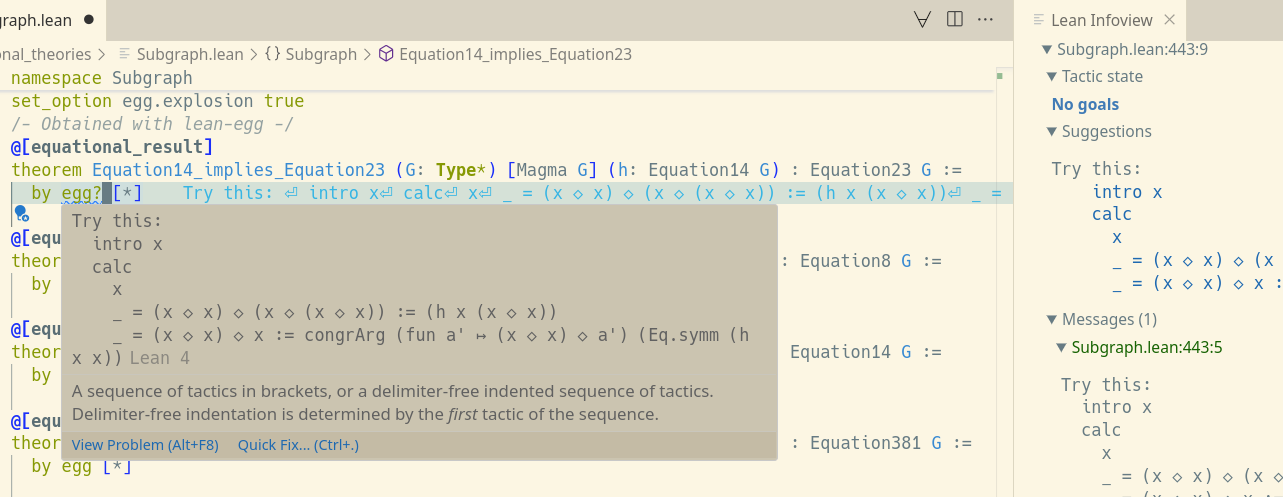
\includegraphics[width=0.85\textwidth]{screenshot-egg.png}
  \caption{An example of the use of proof automation with tactics. This shows the egg tactic as it was used to generate (human-readable) equational proofs of positive implications.}
  \label{fig:screenshot-egg}
\end{figure}

In general, integration implies two steps: invoking the decision procedures/ATPs (translating the problem from Lean into the languages and logics they use), and conversely, (re-)constructing the results from the decision procedure as a (persistent) Lean proof.
These two aspects present different challenges, and require different strategies, depending mostly on the kind of proof strategy the decision procedure uses.

For saturation proofs $\ldots$ (TODO: add explanations from \url{https://leanprover.zulipchat.com/#narrow/channel/458659-Equational/topic/Vampire.20-.3E.20Lean/near/478147138})

For equational proofs from external provers (e.g. MagmaEgg), we used also a simple version of reconstruction by (re-)constructing the proofs of equality from an explanation, using congruence lemmas from Lean.
In the case of equational proofs from the \texttt{egg} tactic, these could be converted into a series of \texttt{calc} steps, documenting the explicit calculation, using the \texttt{calcify} tactic\footnote{\url{https://github.com/nomeata/lean-calcify}}.

In general, we have observed that there are multiple ways of integrating decisions procedures within Lean, with different levels of integration.
\begin{enumerate}
    \item Using a Lean tactic, which calls a decision procedure written in Lean (like \texttt{aesop} or \texttt{duper}).
    \item Using a Lean tactic, which calls an existing (external) ATP and reconstructs a proof term from the ATP's result (like \texttt{bv\_decide} or \texttt{egg}).
    \item\label{external} Using an external script which calls an existing ATP and generates a source file \texttt{.lean} which captures the result explicitly.
\end{enumerate}

This project primarily used the least integrated approach, (Option \ref{external}), as it was fastest and required no dependencies on the other contributors.
This also has drawbacks: primarily, while the upfront effort is lower, the effort to use is higher than with a tactic, once the tactic is developed.
It also makes integration with larger code bases more difficult: in this project the (mathematical) dependencies were by design very minimal, magmas are simple, and we built our own definitions for them.
For example, integration with the typeclass system becomes much more difficult when working with more complex mathematical objects that build on multiple, nested layers of structure in non-trivial ways.
In that case, for example, tactics need to synthesize typeclass instances, deal with diamonds and different notions of equivalence~\cite{DBLP:conf/mkm/Wieser23}.

\paragraph{Semi-Automated Counterexample Guidance}

Another use of ATPs has been in a semi-automatic fashion, to find counter-examples.
The general strategy was to use ATPs to find counter-examples to implications by building magmas iteratively.
If we want to build a counterexample to $l \vdash l'$, we want to construct a magma where $l$ holds but $l'$ does not.
In this method, we iteratively strengthen a construction with additional hypotheses, and use the ATP to check whether these hypotheses are not too strong (to imply $l'$) or unsound (to disallow $l$).

TODO: this should also be expanded more, at least with references to some of the constructions in other chapters.

While equational reasoning can also be used in a semi-automatic fashion to prove equations~\cite{DBLP:journals/pacmpl/KoehlerGBGTS24}, the positive implications in the main implication graph of project were all simple enough that we did not need a semi-automatic approach for them.
TODO: discuss guided search in the finite implications or the Higman-Neumann work Jose Brox has done.

TODO: maybe add a screenshot here of the workflow of using a seed to find counterexamples with prover9 or vampire?

\subsection{Empirical Results}

Finally, we report some empirical results from use of ATPs for this project, in terms of performance.
The aim of this section is not to be a careful evaluation and benchmark comparison of the different ATPs; instead, we present our work here as a more informal ``field report'' documenting our experiences.
In particular, we don't believe we can draw firm conclusions about the overall capabilities of the different ATPs.
Rather, this serves as a use-case documenting the experience of (mostly) novice users.

TODO: throw a couple of "benchmarking" tables for the same ATP with different parameters and for different ATPs, talk about some relative gains in time (changing parameters we saw a 500 times speedup on this particular problem), etc. This is knowledge I think we have gained to some extent, and certainly I would have been glad to receive this kind of hints before we started!''.  Then leave it as an interesting open problem to properly develop and measure benchmarks for ATPs based on this project.

TODO: Any comparative study of semi-automated methods with fully automated ones? In principle, the semi-automated approach could be more automated using a script or "agent" to call various theorem provers. See \href{https://leanprover.zulipchat.com/#narrow/stream/458659-Equational/topic/A.20magma.20of.20order.20.3C.2013.20-.20for.20Equation2531.3F}{this discussion}.

Note: when evaluating the performance of any particular automated implication tool, we should do a fresh run on the entire base of implications, rather than rely on whatever implications produced by the tool remain in the Lean codebase by the time of writing the paper. This is because (a) many of the previous runs focused only on those implications that were not already ruled out by earlier contributions, and (b) some pruning has been applied subsequent to the initial runs to improve compilation performance. Of course, these runs would not need to be added to the (presumably optimized) codebase at that point, but would be purely for the purpose of gathering performance statistics. More discussion \href{https://leanprover.zulipchat.com/#narrow/stream/458659-Equational/topic/RECORDS.20REQUEST.3A.20data.20and.20performance.20automated.20run.20metrics}{here}.

See \href{https://leanprover.zulipchat.com/#narrow/channel/458659-Equational/topic/1516.20-.3E.20255/near/481547543}{this discussion} on the value of using different ATPs and setting run time parameters etc. at different values.

What are the hardest implications to prove?  See \href{https://leanprover.zulipchat.com/#narrow/channel/458659-Equational/topic/What.20are.20the.20hardest.20positive.20implications.20for.20an.20ATP.3F}{this discussion}.

Make a note of the possible alternate strategy to prove implications outlined \href{https://leanprover.zulipchat.com/#narrow/stream/458659-Equational/topic/Ideas.20for.20unknown.20implications}{here}.
